\documentclass[11pt,a4paper,ngerman]{article}
\usepackage[bottom=2.5cm,top=2.5cm]{geometry} 
\usepackage{babel}
\usepackage[utf8]{inputenc} 
\usepackage[T1]{fontenc} 
\usepackage{ae} 
\usepackage{amssymb} 
\usepackage{amsmath}
\usepackage{amsthm} 
\usepackage{graphicx}
\usepackage{fancyhdr}
\usepackage{fancyref}
\usepackage{enumerate}
\usepackage{listings}
\usepackage{xcolor}
\usepackage{paralist}
\usepackage{tabularx}

\usepackage[pdftex, bookmarks=false, pdfstartview={FitH}, linkbordercolor=white]{hyperref}
\usepackage{fancyhdr}
\pagestyle{fancy}
\fancyhead[C]{Numerik I}
\fancyhead[L]{Übung 6}
\fancyhead[R]{SoSe 2013}
\fancyfoot{}
\fancyfoot[L]{}
\fancyfoot[C]{\thepage \hspace{1px} of \pageref{LastPage}}
\renewcommand{\footrulewidth}{0.5pt}
\renewcommand{\headrulewidth}{0.5pt}
\setlength{\parindent}{0pt} 
\setlength{\headheight}{0pt}

\date{Tutor : Christina Schulz}
\title{Übung 6}
\author{Max Wisniewski, Alexander Steen}


%%
%% Enviroments for proofs and lemmas
%%
\newtheorem{lemma}{\bfseries Claim}

\begin{document}

\lstset{language=Pascal, basicstyle=\ttfamily\fontsize{10pt}{10pt}\selectfont\upshape, commentstyle=\rmfamily\slshape, keywordstyle=\rmfamily\bfseries, breaklines=true, frame=single, xleftmargin=3mm, xrightmargin=3mm, tabsize=2, mathescape=true}

\renewcommand{\figurename}{Figure}

\maketitle
\thispagestyle{fancy}

%%%%%%%%%%%%%%%%%%%%%%%%%%%%%%
%% Aufgabe 1 %%%%%%%%%%%%%%%%
%%%%%%%%%%%%%%%%%%%%%%%%%%%%%%
\subsection*{Aufgabe 1}

Sei $S_\Delta^m$ der Raum der Splines $m$-ter Ordnung zum Gitter $\Delta = \{ t_0 , ..., t_n \}$.

Zeigen Sie
\begin{equation*}
    \dim S_\Delta^m = n + m.
\end{equation*}

\textbf{Beweis:}\\

Der Beweis steht schon fast vollständig im Skript.

Eine Funktion
\begin{equation*}
    f \in S_\Delta^m = \{ f \in C^{m-1}[a,b] \, | \, v|_{I_k} = p_k \in \mathcal{P}_m\}
\end{equation*}
wird, wie man sieht, durch $n$ Polynome beschrieben, die alle Grad $k$ haben.
Wir können $f$ also durch $n \cdot (m+1)$ Koeffizienten beschreiben.\\

Da die Funktion im Übergang $m-1$ fach stetig differenzierbar sein muss, gilt nach Übergangsbedingung,
dass $p_k^j(x_k) = p_{k+1}^(j)(x_k)$ für alle $0 \leq j < m$ und $0 \leq k < n$.\\

Wir verlieren nun für jede der Bedingungen einen Freiheitsgrad, da in den Punkten $t_k$ immer
gelten muss, dass die $i$-te Ableitung auf beiden angrenzenden Funktionen je eine Variable fest setzen
wird (wie wir bei der Interpolation vorher gesehen haben).

Pro Polynom ''verlieren'' wir so also $m$ Koeffizienten, die wir frei wählen können. Dies gilt nicht für
$t_0$ und $t_n$ da wir nicht auf die Rahmenbedingung zum Nachbarn achten müssen. Die restlichen
Koeffizienten können immer noch frei gewählt werden, da es sich beim Polynomring um einen Vektorraum handelt.

Folglich erhalten wir
\begin{equation*}
    \dim S_\Delta^m = \underbrace{n(m+1)}_\text{\#Mögliche Koeffizienten} - \underbrace{m(n-1)}_\text{stetig im Gitter} = n + m
\end{equation*}
\mbox{}\hfill$\square$

\subsection*{Aufgabe 2}

\subsubsection*{(a)}

Implementieren Sie eine Matlab Function für das Interpolieren/Approxmieren einer Funktion mit Kubischen Splines.\\

\textbf{Lösung:}\\
Die Funktion benutzt die Berechnungsvorschriften des Skriptes.
Für zwei Eingabelisten $[x_1,\ldots,x_k]$, $[y_1 = f(x_1),\ldots,y_k = f(x_k)]$ 
intepoliert die Funktion mittels kubischen Splines die Funktion $f$ und gibt
deren interpolierte Funktionswerte für die Eingabeliste $t = [t_1, \ldots, t_j]$
zurück. \\
Siehe Dokumentation im Code.

\begin{lstlisting}[basicstyle=\ttfamily\scriptsize\selectfont\upshape,language=matlab,numbers=left,]
%% Gibt ein Gitter X = {x_1, ..., x_n} vor mit Werten
%% Y = {y_1 = f(x_1) , .... , y_n = f(x_n)} und berechnet
%% die Interpolierte Funktion an den Punkten XPos = { t_1 ... t_m }
%% wobei wir t_i < t_(i+1) annehmen (wichtig!)
%% R ist ein Vektor mit Randbedingungen
%% in diesem Fall die Ableitung in x_0 und x_n
function YPos = cub2 (X , Y, R , XPos)
    %% Anzahl der Intervalle
    n = length(X) - 1;

    %% Losen der linearen Gleichung Mc = b
    beta = zeros(1,n+1);
    M = 2 * eye(n+1);
    
    %% Randbedingung (Hermite Gleichung
    beta(1) = 6 * ((Y(2) - Y(1))/(X(2)-X(1))-R(1))/(X(2) - X(1));
    beta(n+1) = 6 * (R(2) - (Y(n+1) - Y(n))/(X(n+1) - X(n)))/(X(n+1)-X(n));

    for i = 2:n
        fa = (Y(i) - Y(i-1))/(X(i) - X(i-1));
        fb = (Y(i+1) - Y(i))/(X(i+1) - X(i));
        beta(i) = 6*(fb - fa)/(X(i+1) - X(i-1));
    end

    %% Matrix M mit mu und lambda wie im skript
    M(1,2) = 1; %% lambda_0 ist immer 1
    for i = 1:(n-1)
        M(i+1,i+2) = (X(i+2)-X(i+1))/(X(i+2) - X(i));
    end

    M(n+1,n) = 1; %% mu_n ist immer 1
    for i = 1:(n-1)
        M(i+1,i) = (X(i+1) - X(i))/(X(i+2) - X(i));
    end
    c = linsolve(M, beta');
    
    %% Berechne b's
    b = zeros(1,n);
    for i = 1:n
        h2 = X(i+1) - X(i);
        f2 = (Y(i+1) - Y(i))/h2;
        b(i) = f2 - h2/6*(2 * c(i) + c(i+1));
    end

    %% Berechne d's
    d = zeros(1,n);
    for i = 1:n
        d(i) = (c(i+1) - c(i))/(X(i+1)-X(i));
    end
   
    %% Auswertung der Eingabestellen t_i
    %% Dazu: In welchem Intervall liegt t_i?
    %% Dann: Auswertung des kubisches Polynoms des Intervalls
    %% mit Taylor
    curPoly = 1;
    m = length(XPos);
    YPos = zeros(1,m);
    for i = 1:m
        %% XPos innerhalb des Intervalls
        while XPos(i) > X(curPoly+1)
            curPoly = curPoly + 1;
        end
        %% Auswertung mit Taylor
        YPos(i) = polyval([(d(curPoly)/6) (c(curPoly)/2) b(curPoly) Y(curPoly)], (XPos(i) - X(curPoly)));
    end
    return;
\end{lstlisting}

\subsubsection*{(b)}
Testen des Programms an der Funktion $f = \sqrt{1,5 + x}$ auf dem Intervall $I = [-1,1]$
mit äquidistanten Knoten.\\

\textbf{Lösung:}\\
Es gilt $f(-\frac{5}{16} \pi) \approx 0.7198974$.

\begin{tabular}{c|c|c||c}
$i$ & $n$ & $ca. \phi_n(f)(-\frac{5}{16} \pi)$ & ca. Fehler \\
\hline \hline
1 & 1 & 0.707626 & 0.012271 \\
2 & 16 & 0.7098757 & 0.010021 \\
3 & $4^3$ &  0.7167205 &  0.0031769 \\
4 & $4^4$ & 0.719831 & $6.665823\cdot 10^{-5}$ \\
5 & $4^5$ & 0.7198974 &  $1.6561232\cdot 10^{-9}$ \\
6 & $4^6$ & 0.7198974 &  $1.2212453\cdot 10^{-15}$ \\
7 & $4^7$ &  0.71989742 & $\approx 0$ \\
8 & $4^8$ & ... & ...
\end{tabular}

Wie wir sehen, ist der absolute Fehler bereits bei $i = 7$ nach der Maschinengenauigkeit von MATLAB gleich 0 (der tatsächliche Fehler also sehr klein).

\subsection*{Aufgabe 3}

Zeichnen Sie ihre Hand nach. Interpolieren Sie die gewählten Punkte mittels Kubischen Splines und natürlichen Randbedingungen
und interpolieren Sie es mittels pchip. Berechnen Sie es einmal über $x$ und einmal über $y$. Welchen unterschied
haben die beiden Verfahren.\\

\textbf{Lösung:}\\

Die Aufnahmepunkte wurden wie in der Aufgabe beschrieben erhoben und interpoliert. Abbildung~\ref{abb:1} zeigt die Interpolation der x-Koordinaten, Abbildung~\ref{abb:2} die Interpolation der y-Koordinaten; jeweils durch  die MATLAB-Funktion \texttt{pchip} und die MATLAB-Funktion \texttt{spline}\footnote{Unser Programm aus Aufgabe 2 wurde erst relativ spät fertig; darum haben wir schon vorher diese Aufgabe gelöst -- die Ergebnisse sollten aber die gleichen sein.}.
Leider war uns nicht klar, wie wir der Funktion \texttt{pchip} bzw. \texttt{spline} die ''natürlichen Randbedingungen'' übergeben sollen, da diese Funktion diese Eingabeparameter nicht vorsehen.

\begin{figure}[h]
\centering
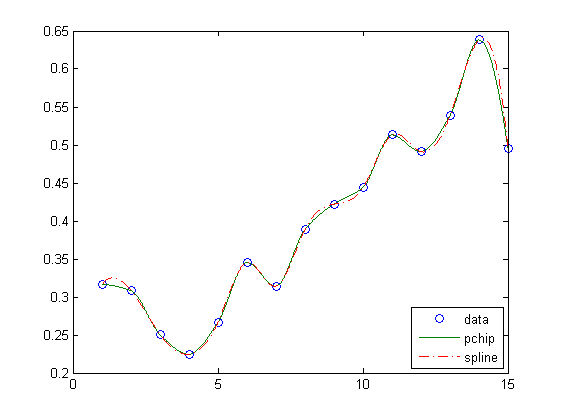
\includegraphics[width=0.8\textwidth]{plotX.png}
\caption{Interpolation der $x$-Koordinaten\label{abb:1}}
\end{figure}

\begin{figure}[h]
\centering
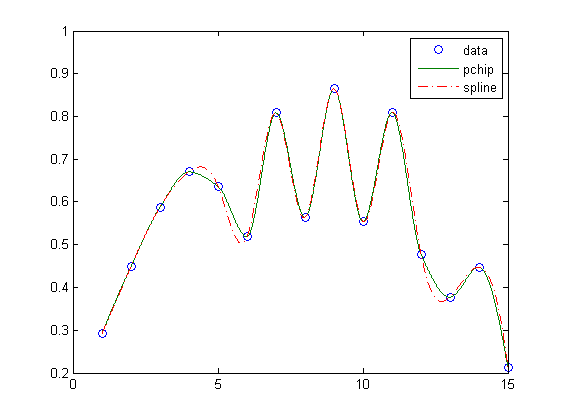
\includegraphics[width=0.8\textwidth]{plotY.png}
\caption{Interpolation der $y$-Koordinaten\label{abb:2}}
\end{figure}

\textbf{Beobachtungen}: Die Interpolation durch \texttt{spline} wirkt glatter bzw. ''geschmeidiger'',
macht also weniger starke bzw. enge Kurven. Die Kurven, die von \texttt{pchip} erzeugt werden, haben
weniger ''ausladende Schlaufen'', also keine kleine Oszillation um Datenpunkte.

\textbf{Erklärung}: Die beiden Methoden scheinen sich sehr stark zu ähneln. Der größte Unterschied ist,
dass \texttt{spline} die (stückweisen) Kurven so auswählt, dass die zweite Ableitung stetig ist.
Dies ist bei \texttt{pchip} nicht der Fall.
\label{LastPage}
\end{document}
